\hypertarget{question-1}{%
\section{Question 1}\label{question-1}}

\hypertarget{question-1.1}{%
\section{Question 1.1}\label{question-1.1}}

\begin{python}[language=Python]
import numpy as np 
import pandas as pd 
import matplotlib.pyplot as plt 
plt.style.use('seaborn-v0_8-whitegrid')
%matplotlib inline
\end{python}

\begin{python}[language=Python]
px = pd.read_csv("../../Data/priceData.csv")
logpx = np.log(px["SPX Index"])
logpx_plot = pd.concat([px["date"], logpx], axis=1)
logpx_plot.plot(x="date", y="SPX Index")
plt.xlabel("date")
plt.ylabel("SPX Index")
\end{python}

\begin{python}
Text(0, 0.5, 'SPX Index')
\end{python}

\begin{figure}[h]
\centering
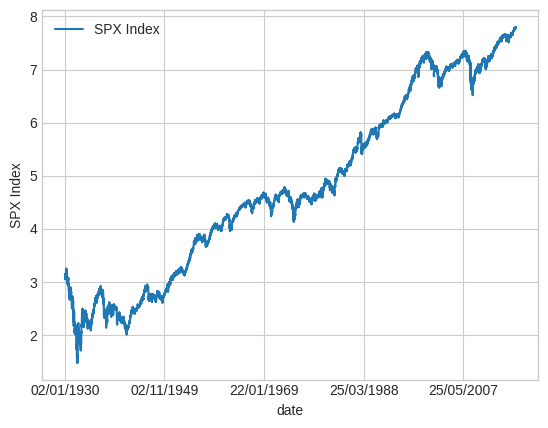
\includegraphics[scale=0.75]{ProcessingStockPriceData_files/ProcessingStockPriceData_3_1.png}
\caption{png}
\end{figure}

\hypertarget{question-1.2}{%
\section{Question 1.2}\label{question-1.2}}

\begin{python}[language=Python]
plt.figure()
logpx_rolling_mean = logpx.ffill().rolling(252, min_periods=1).mean() 
logpx_rolling_mean_plot = pd.concat([px["date"], logpx_rolling_mean], axis=1)
logpx_rolling_mean_plot.plot(x="date", y="SPX Index")
plt.show()

plt.figure()
logpx_rolling_std = logpx.ffill().rolling(252, min_periods=1).std()
logpx_rolling_std_plot = pd.concat([px["date"], logpx_rolling_std], axis=1)
logpx_rolling_std_plot.plot(x="date", y="SPX Index")
plt.show()
\end{python}

\begin{python}
<Figure size 800x550 with 0 Axes>
\end{python}

\begin{figure}[h]
\centering
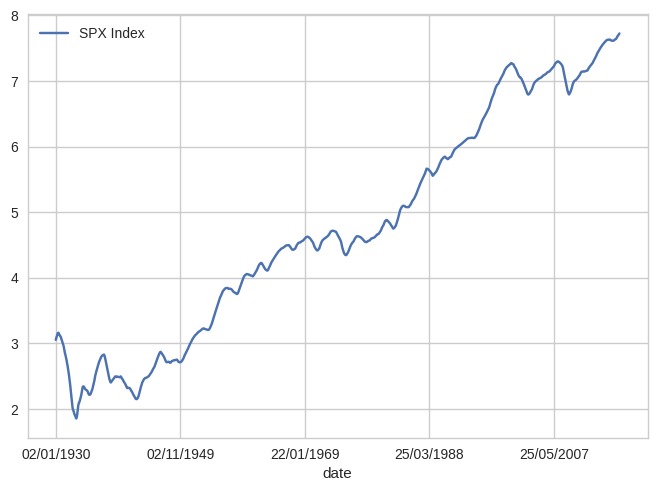
\includegraphics[scale=0.75]{ProcessingStockPriceData_files/ProcessingStockPriceData_5_1.png}
\caption{png}
\end{figure}

\begin{python}
<Figure size 800x550 with 0 Axes>
\end{python}

\begin{figure}[h]
\centering
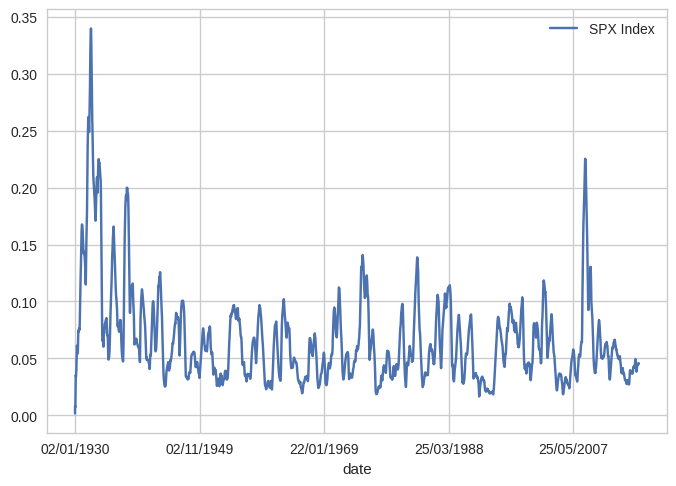
\includegraphics[scale=0.75]{ProcessingStockPriceData_files/ProcessingStockPriceData_5_3.png}
\caption{png}
\end{figure}

\hypertarget{question-1.3}{%
\section{Question 1.3}\label{question-1.3}}

\begin{python}[language=Python]
logret = logpx.ffill().diff()
logret_plot = pd.concat([px["date"], logret], axis=1)
logret_plot.plot(x="date", y="SPX Index")

simpret = px["SPX Index"].ffill().pct_change()
simpret_plot = pd.concat([px["date"], simpret], axis=1)
simpret_plot.plot(x="date", y="SPX Index")
\end{python}

\begin{python}
<Axes: xlabel='date'>
\end{python}

\begin{figure}[h]
\centering
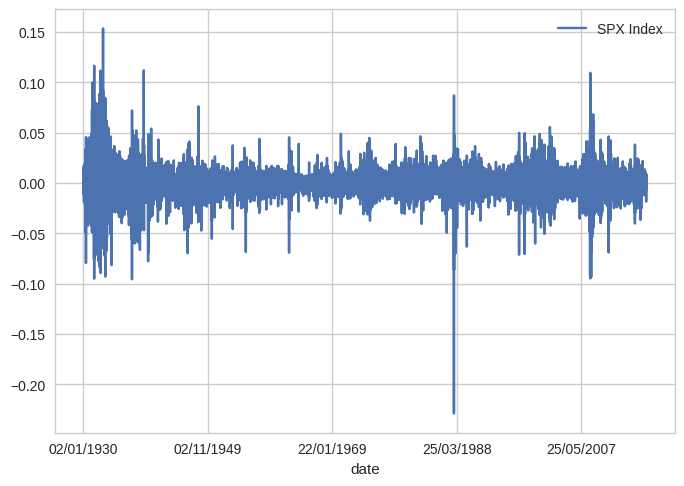
\includegraphics[scale=0.75]{ProcessingStockPriceData_files/ProcessingStockPriceData_7_1.png}
\caption{png}
\end{figure}

\begin{figure}[h]
\centering
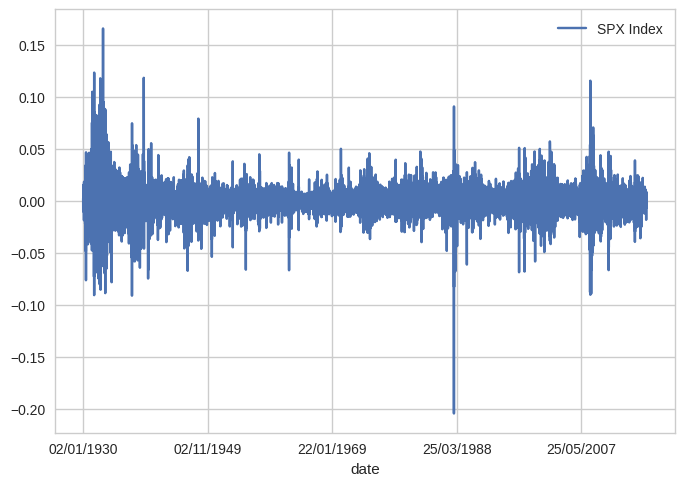
\includegraphics[scale=0.75]{ProcessingStockPriceData_files/ProcessingStockPriceData_7_2.png}
\caption{png}
\end{figure}

\begin{python}[language=Python]
plt.figure()
logret_rolling_mean = logret.rolling(252, min_periods=1).mean() 
logret_rolling_mean_plot = pd.concat([px["date"], logret_rolling_mean], axis=1)
logret_rolling_mean_plot.plot(x="date", y="SPX Index")
plt.show()

plt.figure()
logret_rolling_std = logret.rolling(252, min_periods=1).std() 
logret_rolling_std_plot = pd.concat([px["date"], logret_rolling_std], axis=1)
logret_rolling_std_plot.plot(x="date", y="SPX Index")
plt.show()

plt.figure()
simpret_rolling_mean = simpret.rolling(252, min_periods=1).mean() 
simpret_rolling_mean_plot = pd.concat([px["date"], logret_rolling_mean], axis=1)
simpret_rolling_mean_plot.plot(x="date", y="SPX Index")
plt.show()

plt.figure()
simpret_rolling_std = simpret.rolling(252, min_periods=1).std() 
simpret_rolling_std_plot = pd.concat([px["date"], simpret_rolling_std], axis=1)
simpret_rolling_std_plot.plot(x="date", y="SPX Index")
plt.show()
\end{python}

\begin{python}
<Figure size 800x550 with 0 Axes>
\end{python}

\begin{figure}[h]
\centering
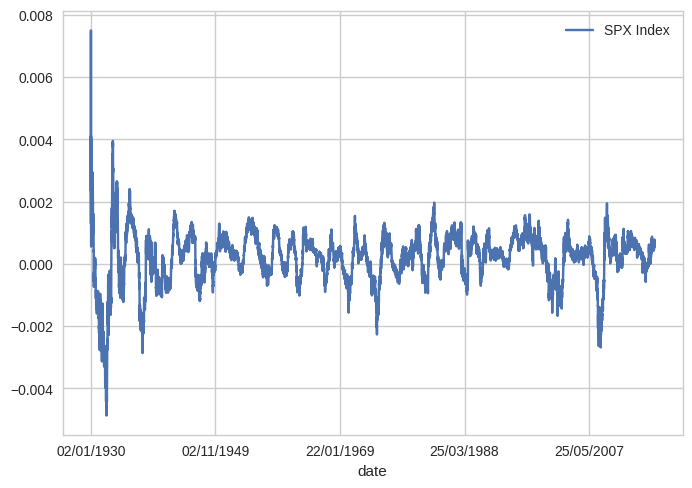
\includegraphics[scale=0.75]{ProcessingStockPriceData_files/ProcessingStockPriceData_8_1.png}
\caption{png}
\end{figure}

\begin{python}
<Figure size 800x550 with 0 Axes>
\end{python}

\begin{figure}[h]
\centering
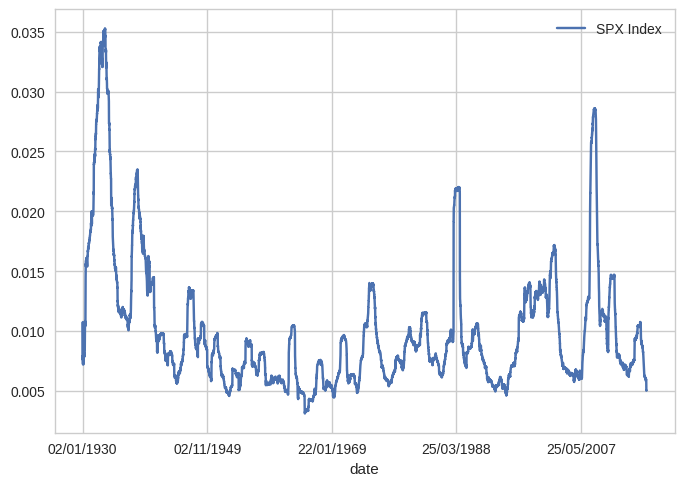
\includegraphics[scale=0.75]{ProcessingStockPriceData_files/ProcessingStockPriceData_8_3.png}
\caption{png}
\end{figure}

\begin{python}
<Figure size 800x550 with 0 Axes>
\end{python}

\begin{figure}[h]
\centering
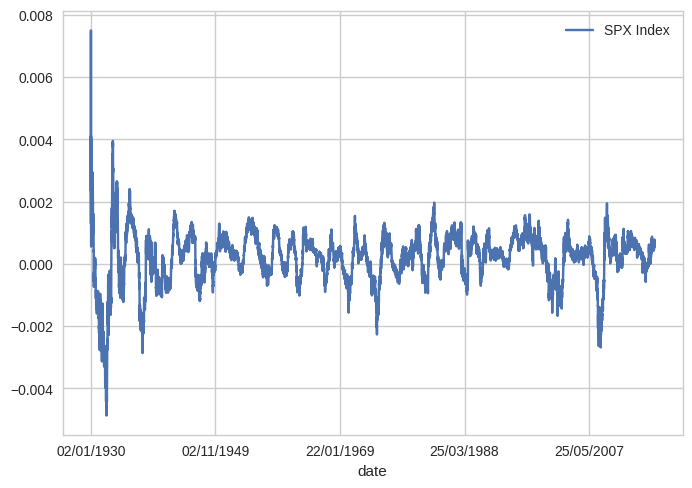
\includegraphics[scale=0.75]{ProcessingStockPriceData_files/ProcessingStockPriceData_8_5.png}
\caption{png}
\end{figure}

\begin{python}
<Figure size 800x550 with 0 Axes>
\end{python}

\begin{figure}[h]
\centering
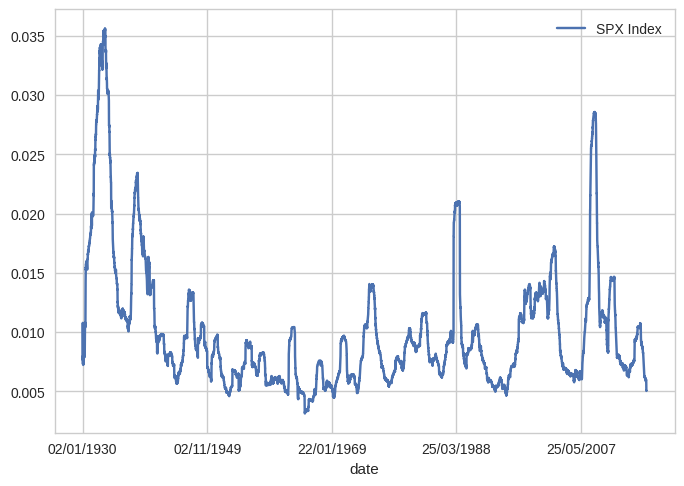
\includegraphics[scale=0.75]{ProcessingStockPriceData_files/ProcessingStockPriceData_8_7.png}
\caption{png}
\end{figure}

\hypertarget{question-1.4}{%
\section{Question 1.4}\label{question-1.4}}

\begin{python}[language=Python]
from scipy import stats
jb_stats = stats.jarque_bera(px["SPX Index"].dropna())
print(jb_stats.pvalue)
print(jb_stats.statistic)
\end{python}

\begin{python}
0.0
9841.005017016492
\end{python}

\hypertarget{question-1.5}{%
\section{Question 1.5}\label{question-1.5}}

Day 1: Day 2: Day 3: \$1 \$2 \$1\\
Simp Returns: Day 1: Day 2: Day 3: 0 1 -0.50

Log Returns: Day 1: Day 2: Day 3: 0 0.69 -0.69

Looking at this we can see that logarithmic percentage changes are
addative rather than mutiplicative therefore it removes directional bias
within our data.

\hypertarget{question-1.6}{%
\section{Question 1.6}\label{question-1.6}}

When analyzing rapodly changing assets over shorter time frames with
smaller overall changes the regular simple returns will approximate
closely to that of the log returns while maintaining simplicity. This
can be important in fast acting systems as the log can be a
computationally expensive operation to compute.
